\documentclass[11pt,a4paper]{article}

\usepackage[utf8]{inputenc}
\usepackage[T5]{fontenc}
\usepackage{amsmath, amssymb, amsfonts}
\usepackage[a4paper, top=22mm, bottom=22mm, left=25mm, right=20mm]{geometry}
\usepackage{graphicx}
\usepackage{xcolor}
\usepackage{tikz}
\usetikzlibrary{shapes.geometric, arrows.meta, positioning, calc, fit, backgrounds, shadows}
\usepackage{listings}
\usepackage{fancyhdr}
\usepackage{booktabs, tabularx, array}
\usepackage{colortbl}
\usepackage{subcaption}
\usepackage{float}
\usepackage[unicode, colorlinks=true, linkcolor=primary, citecolor=secondary, urlcolor=secondary]{hyperref}

% Cho phép LaTeX co giãn khoảng cách từ linh hoạt để triệt tiêu toàn bộ Overfull / Underfull \hbox
\emergencystretch=3em
\tolerance=2000
\hbadness=10000
\hfuzz=2pt

% Định nghĩa hệ màu chuẩn UET
\definecolor{primary}{RGB}{0, 45, 98}        % UET Navy Blue
\definecolor{secondary}{RGB}{0, 102, 153}    % Bright Blue
\definecolor{accent}{RGB}{180, 25, 25}       % Dark Red
\definecolor{codebg}{RGB}{248, 249, 250}     % Code background
\definecolor{logbg}{RGB}{250, 250, 250}      % Terminal log background
\definecolor{commentgreen}{RGB}{0, 128, 0}
\definecolor{keywordblue}{RGB}{0, 0, 204}
\definecolor{stringred}{RGB}{163, 21, 21}
\definecolor{boxbg}{RGB}{240, 245, 253}
\definecolor{borderblue}{RGB}{180, 205, 235}

% Định dạng tiêu đề các mục (Section Headings)
\makeatletter
\renewcommand{\section}{\@startsection{section}{1}{\z@}%
  {-3.5ex \@plus -1ex \@minus -.2ex}%
  {2.3ex \@plus.2ex}%
  {\normalfont\large\bfseries\color{primary}}}
\renewcommand{\subsection}{\@startsection{subsection}{2}{\z@}%
  {-3.25ex\@plus -1ex \@minus -.2ex}%
  {1.5ex \@plus .2ex}%
  {\normalfont\normalsize\bfseries\color{secondary}}}
\renewcommand{\subsubsection}{\@startsection{subsubsection}{3}{\z@}%
  {-3.25ex\@plus -1ex \@minus -.2ex}%
  {1.5ex \@plus .2ex}%
  {\normalfont\normalsize\bfseries\color{primary}}}
\makeatother

% Thiết lập Header và Footer theo chuẩn mẫu báo cáo
\setlength{\headheight}{15pt}
\pagestyle{fancy}
\fancyhf{}
\fancyhead[L]{\small\textit{ĐHQGHN - Trường ĐH Công nghệ}}
\fancyhead[R]{\small\textit{Báo cáo bài tập: Localization, Nav2 \& YOLOv8 trên TurtleBot 4}}
\fancyfoot[C]{\thepage}
\renewcommand{\headrulewidth}{0.4pt}

% Đổi tên các thành phần sang tiếng Việt chuẩn
\renewcommand{\contentsname}{Mục lục}
\renewcommand{\figurename}{Hình}
\renewcommand{\tablename}{Bảng}
\renewcommand{\lstlistingname}{Đoạn mã}

% Cấu hình listings cho Code và Terminal Logs
\lstset{
  basicstyle=\ttfamily\scriptsize,
  backgroundcolor=\color{codebg},
  frame=single,
  rulecolor=\color{black!20},
  numbers=left,
  numberstyle=\tiny\color{gray},
  stepnumber=1,
  numbersep=6pt,
  showstringspaces=false,
  breaklines=true,
  breakatwhitespace=true,
  tabsize=2,
  commentstyle=\color{commentgreen},
  keywordstyle=\color{keywordblue}\bfseries,
  stringstyle=\color{stringred}
}

\newcolumntype{Y}{>{\centering\arraybackslash}X}
\newcolumntype{L}[1]{>{\raggedright\arraybackslash}p{#1}}
\newcolumntype{R}{>{\raggedright\arraybackslash}X}

\begin{document}

% ==============================================================================
% TRANG BÌA (COVER PAGE) VỚI KHUNG VIỀN KÉP THEO CHUẨN MẪU BÁO CÁO UET
% ==============================================================================
\begin{titlepage}
  \begin{tikzpicture}[remember picture, overlay]
    \draw[line width=1.5pt, color=primary] 
      ($(current page.north west)+(15mm,-15mm)$) rectangle ($(current page.south east)+(-15mm,15mm)$);
    \draw[line width=0.5pt, color=primary] 
      ($(current page.north west)+(16.5mm,-16.5mm)$) rectangle ($(current page.south east)+(-16.5mm,16.5mm)$);
  \end{tikzpicture}

  \begin{center}
    \vspace*{5mm}
    {\large\bfseries ĐẠI HỌC QUỐC GIA HÀ NỘI}\\[4pt]
    {\large\bfseries TRƯỜNG ĐẠI HỌC CÔNG NGHỆ}\\[18pt]

    \includegraphics[width=3.2cm]{figures/uet_logo.png}\\[20pt]

    {\Large\bfseries BÁO CÁO THỰC HÀNH}\\[14pt]
    
    {\Huge\bfseries\color{primary} ĐIỀU KHIỂN ROBOT DI ĐỘNG}\\[6pt]
    {\Huge\bfseries\color{primary} TURTLEBOT 4}\\[14pt]
    
    {\large\bfseries ĐỊNH VỊ BẢN ĐỒ (LOCALIZATION), ĐIỀU HƯỚNG TỰ ĐỘNG VỚI NAV2}\\[4pt]
    {\large\bfseries VÀ NHẬN DIỆN VẬT THỂ BẰNG CAMERA OAK-D KẾT HỢP YOLOv8}\\[40pt]

    \vfill

    \begin{tabular}{ll}
      \textbf{Sinh viên thực hiện:} & Nguyễn Quang Tuân -- 23020767 \\[6pt]
      \textbf{Giảng viên hướng dẫn:} & PGS.TS. Hoàng Văn Xiêm \\[3pt]
      & CN. Nguyễn Quốc Bảo
    \end{tabular}

    \vspace{25mm}
    {\large\bfseries Hà Nội -- 2026}
    \vspace*{10mm}
  \end{center}
\end{titlepage}

% ==============================================================================
% MỤC LỤC (TABLE OF CONTENTS)
% ==============================================================================
\newpage
\pagenumbering{roman}
\tableofcontents
\newpage
\pagenumbering{arabic}
\setcounter{page}{1}

% ==============================================================================
% MỤC 1: TỔNG QUAN HỆ THỐNG VÀ CẤU TRÚC CHƯƠNG TRÌNH
% ==============================================================================
\section{TỔNG QUAN HỆ THỐNG \& CẤU TRÚC DỰ ÁN}

\subsection{Mục tiêu bài thực hành}
Bài thực hành kế thừa bản đồ 2D Occupancy Grid (\texttt{map.yaml}, \texttt{map.pgm}) đã xây dựng ở tuần trước để giải quyết bài toán tích hợp toàn diện gồm 04 phần trên robot \textbf{TurtleBot 4 Standard} trong môi trường mô phỏng \textbf{Gazebo Fortress}:
\begin{enumerate}
  \item \textbf{Phần 1 -- Khởi chạy Simulation \& Load bản đồ (Localization):} Khởi chạy lại TurtleBot 4 trong đúng môi trường \texttt{warehouse}, bổ sung các mô hình vật thể (người, ghế, bàn), nạp bản đồ \texttt{map.yaml}, khởi chạy AMCL cùng Nav2 và thiết lập vị trí ban đầu (\textit{Initial Pose}) sao cho dữ liệu quét LiDAR \texttt{/scan} trùng khớp hoàn toàn với tường trên bản đồ RViz2.
  \item \textbf{Phần 2 -- Khảo sát và lấy tọa độ mục tiêu trên bản đồ:} Sử dụng công cụ \textit{Publish Point} (\texttt{/clicked\_point}) và \texttt{/amcl\_pose} để xác định, chuyển đổi và lưu tọa độ $(x, y, \text{yaw})$ trong hệ tọa độ \texttt{map} của ít nhất 03 điểm mục tiêu (Goal 1, Goal 2, Goal 3) tại các khu vực khác nhau.
  \item \textbf{Phần 3 -- Lập trình Navigation tự động với Nav2 (Bằng Code):} Viết chương trình ROS 2 Node bằng Python sử dụng thư viện \texttt{nav2\_simple\_commander} cùng giao thức Action \texttt{/navigate\_to\_pose} để tự động điều khiển robot di chuyển tuần tự qua $\text{Goal 1} \to \text{Goal 2} \to \text{Goal 3}$ không va chạm mà không cần dùng chuột đặt goal trên RViz2.
  \item \textbf{Phần 4 -- Nhận diện vật thể từ Camera với YOLO:} Viết ROS 2 Node subscribe ảnh từ camera RGB (\texttt{/oakd/rgb/preview/image\_raw}), chuyển đổi qua \texttt{cv\_bridge} sang OpenCV, đưa qua mô hình \textbf{YOLOv8} (\texttt{yolov8n.pt}) để nhận diện vật thể, vẽ Bounding Box + tên class + độ tự tin lên cửa sổ OpenCV, publish ngược lại lên topic \texttt{/yolo/detections/image} để xem trên RViz2 và in kết quả ra Terminal.
\end{enumerate}

\subsection{Cấu trúc thư mục gói chương trình trong \texttt{src/}}
Toàn bộ mã nguồn được đóng gói chuẩn hóa trong package \texttt{turtlebot4\_practice4}:

\begin{lstlisting}[language=bash]
turtlebot4_ws/src/
|-- turtlebot4_practice4/
|   |-- package.xml                       # Tuyen bo phu thuoc ROS 2 package
|   |-- setup.py                          # Cau hinh 07 console_scripts thuc thi
|   |-- turtlebot4_practice4/
|   |   |-- spawn_yolo_objects.py         # (Phan 1) Them mo hinh nguoi, ghe, ban vao Gazebo
|   |   |-- auto_undock.py                # (Phan 1) Tu dong dieu khien robot roi tram sac
|   |   |-- tf_relay.py                   # (Phan 1) Dong bo TF va mock hardware services
|   |   |-- goal_survey.py                # (Phan 2) Khao sat /clicked_point & /amcl_pose luu JSON
|   |   |-- auto_nav_goals.py             # (Phan 3) Dieu huong tu dong 03 Goals bang Nav2 Code
|   |   |-- yolo_detector.py              # (Phan 4) Nhan dien vat the Camera OAK-D + YOLOv8
|   |   `-- check_topics.py               # Kiem tra tu dong cac topic cam bien
|   |-- launch/
|   |   |-- sim_robot.launch.py           # Launch Gazebo + TurtleBot 4 Standard (co OAK-D)
|   |   |-- sim_localization.launch.py    # Launch AMCL + Map Server + RViz2
|   |   `-- sim_navigation.launch.py      # Launch tich hop: Sim + Objects + AMCL + Nav2 + YOLO
|   |-- config/
|   |   |-- surveyed_goals.json           # Toa do (x, y, yaw) cua 03 Goals khao sat o Phan 2
|   |   |-- localization_params.yaml      # Tham so bo loc hat AMCL va Map Server
|   |   |-- nav2_params.yaml              # Costmaps, DWB Controller, NavFn Planner, BT
|   |   |-- fastdds_udp_only.xml          # Cau hinh FastDDS UDP-only chong deadlock SHM
|   |   `-- turtlebot4_nav2.rviz          # Giao dien RViz2 hien thi Map, Scan, Path & YOLO Image
|   |-- maps/
|   |   `-- map.yaml & map.pgm            # Ban do 2D da xay dung tu bai thuc hanh tuan truoc
|   |-- scripts/
|   |   |-- run_part1_localization.sh     # Script chay Phan 1: Sim + Load Map + AMCL + Nav2
|   |   |-- run_part2_survey_goals.sh     # Script chay Phan 2: Khao sat 03 Goals tren RViz2
|   |   |-- run_part3_auto_nav.sh         # Script chay Phan 3: Tu dong di qua Goal 1 -> 2 -> 3
|   |   |-- run_part4_yolo.sh             # Script chay Phan 4: Node nhan dien YOLOv8
|   |   `-- run_part4_navigation.sh       # Script chay tich hop toan bo Phan 1 -> Phan 4
|   `-- docs/
|       `-- bao_cao_thuc_hanh_04.(md|html|pdf) & report.tex
`-- irobot_create_control/                # Bo dieu khien vi sai cho de iRobot Create 3
\end{lstlisting}

\subsection{Kiến trúc tích hợp 5 tầng của hệ thống}
\begin{figure}[H]
\centering
\resizebox{0.92\textwidth}{!}{%
\begin{tikzpicture}[
  node distance=5mm and 8mm,
  layer/.style={rectangle, draw=primary!80, fill=boxbg, rounded corners=3pt, line width=0.8pt, align=center, inner sep=5pt, text width=14.2cm},
  subnode/.style={rectangle, draw=secondary!70, fill=white, rounded corners=2pt, font=\scriptsize, align=center, inner sep=3.5pt},
  flowarrow/.style={-Stealth, thick, color=primary}
]
  \node[layer] (layer5) {
    \textbf{\color{primary}TẦNG 5: NHẬN THỨC THỊ GIÁC MÁY TÍNH \& ĐIỀU KHIỂN NHIỆM VỤ TỰ ĐỘNG}\\
    \vspace{2pt}
    \begin{tabular}{ccc}
      \tikz\node[subnode, text width=3.85cm]{\textbf{Node \texttt{yolo\_detector.py}}\\\texttt{cv\_bridge} + YOLOv8 (\texttt{yolov8n.pt})}; &
      \tikz\node[subnode, text width=3.85cm]{\textbf{Node \texttt{auto\_nav\_goals.py}}\\Tự hành tuần tự Goal 1 $\to$ 2 $\to$ 3}; &
      \tikz\node[subnode, text width=3.85cm]{\textbf{Node \texttt{goal\_survey.py}}\\Khảo sát \texttt{/clicked\_point} \& \texttt{/amcl\_pose}};
    \end{tabular}
  };

  \node[layer, below=of layer5] (layer4) {
    \textbf{\color{primary}TẦNG 4: NGĂN XẾP ĐIỀU HƯỚNG TỰ ĐỘNG NAVIGATION 2 (Nav2 Stack)}\\
    \vspace{2pt}
    \begin{tabular}{ccc}
      \tikz\node[subnode, text width=3.85cm]{\textbf{bt\_navigator}\\Action \texttt{/navigate\_to\_pose}}; &
      \tikz\node[subnode, text width=3.85cm]{\textbf{planner\_server} (NavFn)\\Quy hoạch đường đi toàn cục \texttt{/plan}}; &
      \tikz\node[subnode, text width=3.85cm]{\textbf{controller\_server} (DWB)\\Điều khiển vận tốc \texttt{/cmd\_vel} 20 Hz};
    \end{tabular}
  };

  \node[layer, below=of layer4] (layer3) {
    \textbf{\color{primary}TẦNG 3: NẠP BẢN ĐỒ TĨNH \& ĐỊNH VỊ MONTE CARLO THÍCH NGHI (Localization)}\\
    \vspace{2pt}
    \begin{tabular}{ccc}
      \tikz\node[subnode, text width=3.85cm]{\textbf{map\_server}\\Nạp \texttt{map.yaml} \& \texttt{map.pgm} lên \texttt{/map}}; &
      \tikz\node[subnode, text width=3.85cm]{\textbf{amcl} (Particle Filter)\\Ước lượng \texttt{/amcl\_pose}, \texttt{/particle\_cloud}}; &
      \tikz\node[subnode, text width=3.85cm]{\textbf{Initial Pose \& Undock}\\Khởi tạo vị trí $(0.35, 0.0, 3.14)$};
    \end{tabular}
  };

  \node[layer, below=of layer3] (layer2) {
    \textbf{\color{primary}TẦNG 2: CẦU NỐI TRUYỀN THÔNG ROS 2 -- GAZEBO \& CÂY TỌA ĐỘ TF (REP-105)}\\
    \vspace{2pt}
    \begin{tabular}{ccc}
      \tikz\node[subnode, text width=3.85cm]{\textbf{ros\_gz\_bridge}\\Bridge \texttt{/scan}, \texttt{/oakd/rgb/...}, \texttt{/odom}}; &
      \tikz\node[subnode, text width=3.85cm]{\textbf{TF Tree Architecture}\\\texttt{map} $\to$ \texttt{odom} $\to$ \texttt{base\_link} $\to$ \texttt{oakd}}; &
      \tikz\node[subnode, text width=3.85cm]{\textbf{FastDDS UDP-only \& \texttt{tf\_relay}}\\Loại bỏ lỗi SHM deadlock \& trễ giờ};
    \end{tabular}
  };

  \node[layer, below=of layer2] (layer1) {
    \textbf{\color{primary}TẦNG 1: MÔ PHỎNG VẬT LÝ GAZEBO FORTRESS \& MÔ HÌNH VẬT THỂ 3D}\\
    \vspace{2pt}
    \begin{tabular}{ccc}
      \tikz\node[subnode, text width=3.85cm]{\textbf{TurtleBot 4 Standard}\\Create 3 + RPLiDAR + Camera OAK-D}; &
      \tikz\node[subnode, text width=3.85cm]{\textbf{Thế giới \texttt{warehouse}}\\Tường, hành lang và các dãy kệ kho}; &
      \tikz\node[subnode, text width=3.85cm]{\textbf{Node \texttt{spawn\_yolo\_objects}}\\Mô hình Người đứng, Ghế tựa, Ghế gấp, Bàn};
    \end{tabular}
  };

  \draw[flowarrow] (layer5) -- (layer4);
  \draw[flowarrow] (layer4) -- (layer3);
  \draw[flowarrow] (layer3) -- (layer2);
  \draw[flowarrow] (layer2) -- (layer1);
\end{tikzpicture}%
}
\caption{Kiến trúc tích hợp Localization (AMCL), Autonomous Navigation (Nav2) và Nhận diện vật thể (Camera OAK-D + YOLOv8)}
\label{fig:system_arch}
\end{figure}

\subsection{Bảng phân tích các Topic và Action cốt lõi}
\begin{table}[H]
\centering
\footnotesize
\setlength{\tabcolsep}{4pt}
\begin{tabularx}{\textwidth}{L{3.7cm}L{4.3cm}L{1.4cm}R}
\toprule
\textbf{\color{primary}Tên Topic / Action} & \textbf{\color{primary}Kiểu Message / Action} & \textbf{\color{primary}Tần số} & \textbf{\color{primary}Vai trò trong bài thực hành} \\
\midrule
\texttt{/map} & \texttt{nav\_msgs/msg/}\newline\texttt{OccupancyGrid} & Transient & Bản đồ lưới 2D nạp từ \texttt{map.yaml} và \texttt{map.pgm} của tuần trước. \\
\rowcolor{boxbg}
\texttt{/scan} & \texttt{sensor\_msgs/msg/}\newline\texttt{LaserScan} & $10\text{ Hz}$ & 640 tia laser từ RPLiDAR dùng cho AMCL đối sánh với tường và Local Costmap. \\
\texttt{/initialpose} & \texttt{geometry\_msgs/msg/}\newline\texttt{PoseWithCovarianceStamped} & Khởi tạo & Đặt vị trí và góc hướng ban đầu của robot trên bản đồ cho AMCL. \\
\rowcolor{boxbg}
\texttt{/amcl\_pose} & \texttt{geometry\_msgs/msg/}\newline\texttt{PoseWithCovarianceStamped} & $10\text{ Hz}$ & Tọa độ định vị thực tế $(x, y, \text{yaw})$ của robot trong hệ tọa độ \texttt{map}. \\
\texttt{/clicked\_point} & \texttt{geometry\_msgs/msg/}\newline\texttt{PointStamped} & Khi click & Tọa độ điểm mục tiêu lấy từ công cụ \textit{Publish Point} trên RViz2 (Phần 2). \\
\rowcolor{boxbg}
\texttt{/navigate\_to\_pose} & \texttt{nav2\_msgs/action/}\newline\texttt{NavigateToPose} & Action & Action Server nhận mục tiêu từ \texttt{auto\_nav\_goals} và trả về cự ly còn lại. \\
\texttt{/oakd/rgb/preview/}\newline\texttt{image\_raw} & \texttt{sensor\_msgs/msg/Image} & $15\text{--}30\text{ Hz}$ & Luồng ảnh màu RGB từ camera OAK-D trên robot (đầu vào của Phần 4). \\
\rowcolor{boxbg}
\texttt{/yolo/detections/}\newline\texttt{image} & \texttt{sensor\_msgs/msg/Image} & $15\text{--}30\text{ Hz}$ & Ảnh đầu ra đã vẽ Bounding Box, tên class, độ tự tin và HUD để xem trên RViz2. \\
\texttt{/yolo/detections/}\newline\texttt{summary} & \texttt{std\_msgs/msg/String} & $15\text{--}30\text{ Hz}$ & Dữ liệu JSON danh sách vật thể phát hiện gửi sang Node điều hướng. \\
\bottomrule
\end{tabularx}
\caption{Danh sách các Topic và Action cốt lõi sử dụng trong 4 phần của bài tập}
\label{tab:topics}
\end{table}

% ==============================================================================
% MỤC 2: PHẦN 1 - KHỞI CHẠY SIMULATION & LOAD BẢN ĐỒ (LOCALIZATION)
% ==============================================================================
\newpage
\section{PHẦN 1 – SIMULATION \& LOAD BẢN ĐỒ (LOCALIZATION)}

\subsection{Khởi chạy môi trường Gazebo và bổ sung các mô hình vật thể 3D}
Hệ thống khởi chạy lại robot \textbf{TurtleBot 4 Standard} (phiên bản đầy đủ có gắn camera OAK-D RGB-D trên tháp cảm biến và RPLiDAR 2D) trong đúng môi trường \texttt{warehouse} mà bài thực hành tuần trước đã sử dụng để quét bản đồ.

Để phục vụ việc phát hiện và nhận diện vật thể bằng camera + YOLO ở Phần 4, node \texttt{spawn\_yolo\_objects.py} được viết để tự động gọi dịch vụ \texttt{ros\_ign\_gazebo create}, nạp 04 mô hình vật thể 3D từ bộ nhớ đệm Ignition Fuel vào các vị trí thông thoáng quanh các điểm mục tiêu (không chắn ngang hành lang di chuyển của xe):

\begin{table}[H]
\centering
\footnotesize
\setlength{\tabcolsep}{4pt}
\begin{tabularx}{\textwidth}{L{3.6cm}L{3.4cm}cccR}
\toprule
\textbf{\color{primary}Tên thực thể Gazebo} & \textbf{\color{primary}Mô hình SDF (Ignition)} & \textbf{\color{primary}$x$ (m)} & \textbf{\color{primary}$y$ (m)} & \textbf{\color{primary}$\text{yaw}$} & \textbf{\color{primary}Vị trí bố trí trong môi trường} \\
\midrule
\texttt{person\_standing\_goal1} & \texttt{casual female/1/}\newline\texttt{model.sdf} & $-3.20$ & $+0.25$ & $0.00$ & Người đứng gần Goal 1 (Hành lang trung tâm) \\
\rowcolor{boxbg}
\texttt{chair\_goal1} & \texttt{chair/3/model.sdf} & $-3.00$ & $-0.55$ & $+0.40$ & Ghế tựa gần Goal 1 (Hành lang trung tâm) \\
\texttt{chair\_goal2} & \texttt{foldable\_chair/3/}\newline\texttt{model.sdf} & $+0.35$ & $+2.85$ & $-1.57$ & Ghế gấp gần Goal 2 (Hành lang phía Bắc) \\
\rowcolor{boxbg}
\texttt{table\_goal2} & \texttt{table/4/model.sdf} & $+1.25$ & $+3.05$ & $-1.57$ & Bàn làm việc gần Goal 2 (Hành lang phía Bắc) \\
\bottomrule
\end{tabularx}
\caption{Danh sách các mô hình vật thể 3D được bổ sung vào môi trường Gazebo \texttt{warehouse}}
\label{tab:spawned_objects}
\end{table}

\subsection{Nạp bản đồ (\texttt{map.yaml}) và khởi chạy Localization (AMCL) cùng Nav2}
Bản đồ \texttt{maps/map.yaml} (độ phân giải $0.03\text{ m/pixel}$, gốc tọa độ $[-15.1, -25.0, 0.0]$) và tệp ảnh lưới chiếm dụng \texttt{maps/map.pgm} được nạp trực tiếp bởi \texttt{map\_server} cùng với bộ định vị hạt thích nghi \texttt{amcl} và toàn bộ ngăn xếp Nav2 thông qua lệnh:
\begin{lstlisting}[language=bash]
./src/turtlebot4_practice4/scripts/run_part1_localization.sh
# Hoac chay truc tiep qua ros2 launch:
ros2 launch turtlebot4_practice4 sim_navigation.launch.py \
    map:=/home/tuan/turtelbot4_ws/src/turtlebot4_practice4/maps/map.yaml \
    world:=warehouse rviz:=true spawn_objects:=true
\end{lstlisting}

\subsection{Kiểm tra và thiết lập vị trí ban đầu (Initial Pose) cho robot}
\begin{enumerate}
  \item \textbf{Tự động rời trạm sạc (Auto Undock):} Khi mới khởi tạo trong Gazebo, robot nằm trên trạm sạc Dock tại $(0, 0, 0)$. Node \texttt{auto\_undock.py} tự động gửi Action \texttt{/undock} để robot lùi ra vị trí thông thoáng tại $x = 0.35\text{ m}, y = 0.00\text{ m}, \text{yaw} = 3.14159\text{ rad}$ ($180^\circ$).
  \item \textbf{Thiết lập Initial Pose chuẩn xác:} Hệ thống tự động công bố bản tin kiểu \texttt{PoseWithCovarianceStamped} lên topic \texttt{/initialpose} với ma trận hiệp phương sai $\sigma_x^2 = 0.25, \sigma_y^2 = 0.25, \sigma_\psi^2 = 0.068$ và gọi dịch vụ \texttt{/request\_nomotion\_update} để AMCL lập tức tính toán biến đổi $\mathbf{T}_{\text{map} \to \text{odom}}$. (Người dùng cũng có thể đặt lại bất kỳ lúc nào bằng nút \textit{2D Pose Estimate} trên RViz2).
  \item \textbf{Xác thực sự trùng khớp trên RViz2:}
  \begin{itemize}
    \item Bản đồ Occupancy Grid hiển thị rõ nét toàn bộ kết cấu tường bao và các dãy kệ hàng.
    \item Vị trí và hướng của mô hình 3D TurtleBot 4 trên RViz2 trùng khớp hoàn toàn với tư thế thực tế trong Gazebo.
    \item Các điểm chấm đỏ của tia quét LiDAR (\texttt{/scan}) \textbf{nằm đè khít lên các đường viền bức tường đen} trên bản đồ tĩnh, đám mây hạt AMCL (\texttt{/particle\_cloud}) hội tụ chặt quanh tâm robot.
  \end{itemize}
\end{enumerate}

\begin{figure}[H]
\centering
\begin{subfigure}[b]{0.56\textwidth}
  \centering
  \includegraphics[width=\textwidth]{figures/rviz_nav2_costmap.png}
  \caption{Giao diện RViz2: Tia LiDAR \texttt{/scan} trùng khớp với tường bản đồ}
  \label{fig:rviz_loc}
\end{subfigure}
\hfill
\begin{subfigure}[b]{0.40\textwidth}
  \centering
  \includegraphics[width=\textwidth]{figures/map_occupancy_grid.png}
  \caption{Bản đồ \texttt{map.pgm} nạp vào \texttt{map\_server}}
  \label{fig:map_pgm}
\end{subfigure}
\caption{Kết quả nạp bản đồ \texttt{map.yaml} và định vị AMCL trên RViz2}
\label{fig:part1_result}
\end{figure}

% ==============================================================================
% MỤC 3: PHẦN 2 - KHẢO SÁT VÀ LẤY TỌA ĐỘ MỤC TIÊU TRÊN BẢN ĐỒ
% ==============================================================================
\newpage
\section{PHẦN 2 – KHẢO SÁT TỌA ĐỘ MỤC TIÊU TRÊN BẢN ĐỒ}

\subsection{Phương pháp khảo sát và công cụ tự động \texttt{goal\_survey.py}}
Để lấy chính xác tọa độ $(x, y, \text{yaw})$ trong hệ tọa độ \texttt{map} của ít nhất 03 điểm mục tiêu (Goal 1, Goal 2, Goal 3), nhóm đã thực hiện kết hợp cả 2 cách theo gợi ý của đề bài và tích hợp vào node \texttt{turtlebot4\_practice4/goal\_survey.py}:
\begin{enumerate}
  \item \textbf{Sử dụng công cụ \textit{Publish Point} trên RViz2 (\texttt{/clicked\_point}):} Khi chọn công cụ \textit{Publish Point} trên thanh công cụ RViz2 và click chuột vào một điểm trên bản đồ, RViz2 xuất bản tin \texttt{geometry\_msgs/msg/PointStamped} trên frame \texttt{map}. Node \texttt{goal\_survey} tự động bắt sự kiện này, trích xuất $(x, y)$ và tự động tính góc hướng $\text{yaw} = \text{atan2}(y - y_{\text{prev}}, x - x_{\text{prev}})$ hướng về điểm mục tiêu.
  \item \textbf{Theo dõi tọa độ định vị hiện tại của robot qua \texttt{/amcl\_pose}:} Node lắng nghe bản tin \texttt{PoseWithCovarianceStamped} từ AMCL trên topic \texttt{/amcl\_pose} và chuyển đổi tứ nguyên Quaternion $(q_x, q_y, q_z, q_w)$ sang góc xoay Euler $\text{yaw}$ quanh trục $Z$:
  \begin{equation}
    \text{yaw} = \text{atan2}\left(2(q_w q_z + q_x q_y), \; 1 - 2(q_y^2 + q_z^2)\right)
  \end{equation}
  \item \textbf{Tự động lưu tệp cấu hình JSON:} Ngay khi click đủ 03 điểm trên RViz2, node tự động lưu danh sách tọa độ vào tệp \texttt{config/surveyed\_goals.json} để Node điều hướng ở Phần 3 nạp trực tiếp.
\end{enumerate}

Lệnh khởi chạy khảo sát Phần 2:
\begin{lstlisting}[language=bash]
./src/turtlebot4_practice4/scripts/run_part2_survey_goals.sh
# Hoac kiem tra truc tiep bang lenh ROS 2 CLI:
ros2 topic echo /clicked_point
ros2 topic echo /amcl_pose
\end{lstlisting}

\subsection{Kết quả ghi nhận tọa độ 03 điểm mục tiêu (Goal 1, Goal 2, Goal 3)}
Bảng dưới đây tổng hợp cả hai bộ tọa độ đã được khảo sát và cấu hình sẵn trong hệ thống (tất cả đều thuộc hệ tọa độ \texttt{map}):

\begin{table}[H]
\centering
\footnotesize
\setlength{\tabcolsep}{4pt}
\begin{tabularx}{\textwidth}{L{2.2cm}RL{2.0cm}L{2.0cm}L{2.8cm}}
\toprule
\textbf{\color{primary}Điểm mục tiêu} & \textbf{\color{primary}Khu vực trên bản đồ (Hệ tọa độ \texttt{map})} & \textbf{\color{primary}Tọa độ $x$ (m)} & \textbf{\color{primary}Tọa độ $y$ (m)} & \textbf{\color{primary}Góc $\text{yaw}$ (rad / độ)} \\
\midrule
\multicolumn{5}{l}{\textbf{\textit{A. Bộ 03 tọa độ khảo sát qua công cụ Publish Point (\texttt{/clicked\_point} $\to$ \texttt{surveyed\_goals.json}):}}} \\
\midrule
\textbf{Initial Pose} & Vị trí xuất phát sau khi rời trạm sạc (Dock) & $+0.35\text{ m}$ & $+0.00\text{ m}$ & $+3.14\text{ rad}$ ($180.0^\circ$) \\
\rowcolor{boxbg}
\textbf{Goal 1} & Điểm khảo sát khu vực Đông -- Bắc 1 trên RViz2 & $+2.99\text{ m}$ & $+1.55\text{ m}$ & $+0.43\text{ rad}$ ($+24.6^\circ$) \\
\textbf{Goal 2} & Điểm khảo sát hành lang phía Bắc trên RViz2 & $+3.49\text{ m}$ & $+5.37\text{ m}$ & $+1.44\text{ rad}$ ($+82.5^\circ$) \\
\rowcolor{boxbg}
\textbf{Goal 3} & Điểm khảo sát khu vực Tây -- Bắc trên RViz2 & $-2.26\text{ m}$ & $+5.18\text{ m}$ & $-3.11\text{ rad}$ ($-178.2^\circ$) \\
\midrule
\multicolumn{5}{l}{\textbf{\textit{B. Bộ 03 tọa độ chuẩn định hướng trực diện vào cụm vật thể YOLO:}}} \\
\midrule
\textbf{Goal 1} & Khu vực hành lang trung tâm (Đối diện Người \& Ghế) & $-1.50\text{ m}$ & $+0.00\text{ m}$ & $+3.14\text{ rad}$ ($180.0^\circ$) \\
\rowcolor{boxbg}
\textbf{Goal 2} & Khu vực hành lang phía Bắc (Đối diện Ghế gấp \& Bàn) & $+0.50\text{ m}$ & $+1.20\text{ m}$ & $+1.57\text{ rad}$ ($+90.0^\circ$) \\
\textbf{Goal 3} & Khu vực nhân viên kho \& Trạm sạc (South-East View) & $+0.35\text{ m}$ & $+0.00\text{ m}$ & $-0.99\text{ rad}$ ($-56.7^\circ$) \\
\bottomrule
\end{tabularx}
\caption{Bảng tọa độ $(x, y, \text{yaw})$ trong hệ tọa độ \texttt{map} của Initial Pose và 03 điểm mục tiêu}
\label{tab:surveyed_goals}
\end{table}

% ==============================================================================
% MỤC 4: PHẦN 3 - LẬP TRÌNH NAVIGATION TỰ ĐỘNG VỚI NAV2 (BẰNG CODE)
% ==============================================================================
\newpage
\section{PHẦN 3 – LẬP TRÌNH NAVIGATION TỰ ĐỘNG VỚI NAV2}

\subsection{Kiến trúc thuật toán của Node \texttt{auto\_nav\_goals.py}}
Thay vì sử dụng công cụ \textit{Nav2 Goal} kéo thả bằng chuột trên RViz2, nhóm đã xây dựng chương trình điều khiển tự động hoàn toàn bằng code Python tại tệp \texttt{turtlebot4\_practice4/auto\_nav\_goals.py}. Chương trình định nghĩa lớp \texttt{TurtleBot4Navigator} kế thừa từ \texttt{BasicNavigator} của thư viện \texttt{nav2\_simple\_commander} (giao tiếp trực tiếp với Action Server \texttt{/navigate\_to\_pose}):

\begin{figure}[H]
\centering
\begin{tikzpicture}[
  node distance=5mm and 8mm,
  stepbox/.style={rectangle, draw=primary, fill=boxbg, rounded corners=3pt, line width=0.8pt, font=\small, align=center, inner sep=5pt, text width=12.5cm},
  arrow/.style={-Stealth, thick, color=primary}
]
  \node[stepbox] (s1) {\textbf{Bước 1 -- Đồng bộ Clock \& Tự động Undock:} Khởi tạo \texttt{use\_sim\_time:=true}, gọi Action \texttt{/undock} đưa robot rời trạm sạc};
  \node[stepbox, below=of s1] (s2) {\textbf{Bước 2 -- Kích hoạt Localization \& Đặt Initial Pose:} Đảm bảo \texttt{map\_server}, \texttt{amcl} ở trạng thái \texttt{[ACTIVE]}, gọi \texttt{setInitialPose(0.35, 0.0, 3.14)} và \texttt{/request\_nomotion\_update}};
  \node[stepbox, below=of s2] (s3) {\textbf{Bước 3 -- Kích hoạt Nav2 Stack \& Nạp danh sách 03 Goals:} Kiểm tra \texttt{planner\_server}, \texttt{controller\_server}, \texttt{bt\_navigator} \texttt{[ACTIVE]} và đọc 03 tọa độ từ \texttt{surveyed\_goals.json}};
  \node[stepbox, below=of s3] (s4) {\textbf{Bước 4 -- Vòng lặp điều hướng tuần tự ($\text{Goal } i = 1 \to 2 \to 3$):}\\Đóng gói \texttt{PoseStamped} (frame \texttt{map}), gọi \texttt{navigator.goToPose(goal\_pose)}, theo dõi \texttt{distance\_remaining} và kết quả YOLO thời gian thực};
  \node[stepbox, below=of s4] (s5) {\textbf{Bước 5 -- Dừng quét YOLO tại đích \& Tổng kết:} Dừng $3.5\text{s}$ tại mỗi Goal để thu thập toàn bộ vật thể phát hiện được và in bảng báo cáo tổng kết hành trình};

  \draw[arrow] (s1) -- (s2);
  \draw[arrow] (s2) -- (s3);
  \draw[arrow] (s3) -- (s4);
  \draw[arrow] (s4) -- (s5);
\end{tikzpicture}
\caption{Lưu đồ thuật toán điều khiển tự hành tuần tự 03 Goals trong \texttt{auto\_nav\_goals.py}}
\label{fig:autonav_flow}
\end{figure}

\subsection{Đoạn mã nguồn cốt lõi điều khiển tự động qua 03 Goals}
\begin{lstlisting}[language=Python, caption={Trích đoạn hàm tạo PoseStamped và vòng lặp điều hướng tuần tự trong \texttt{auto\_nav\_goals.py}}]
def create_pose_stamped(navigator: BasicNavigator, x: float, y: float, yaw: float) -> PoseStamped:
    """Tao PoseStamped tren he toa do map voi goc xoay yaw (radian)."""
    pose = PoseStamped()
    pose.header.frame_id = 'map'
    pose.header.stamp = navigator.get_clock().now().to_msg()
    pose.pose.position.x = float(x)
    pose.pose.position.y = float(y)
    pose.pose.position.z = 0.0
    half_yaw = yaw * 0.5
    pose.pose.orientation.z = math.sin(half_yaw)
    pose.pose.orientation.w = math.cos(half_yaw)
    return pose

# Vong lap tu dong gui tuan tu Goal 1 -> Goal 2 -> Goal 3:
for idx, g in enumerate(goals, 1):
    goal_pose = create_pose_stamped(navigator, g['x'], g['y'], g['yaw'])
    navigator.goToPose(goal_pose)

    while not navigator.isTaskComplete():
        rclpy.spin_once(navigator, timeout_sec=0.05)
        feedback = navigator.getFeedback()
        if feedback:
            distance_remaining = feedback.distance_remaining
            # Kiem tra khoang cach tiep can dich va in log kem ket qua YOLO...
\end{lstlisting}

\subsection{Quy trình thực thi và đánh giá an toàn}
Chạy lệnh thực thi Phần 3:
\begin{lstlisting}[language=bash]
./src/turtlebot4_practice4/scripts/run_part3_auto_nav.sh
# Hoac: ros2 run turtlebot4_practice4 auto_nav_goals --ros-args -p use_sim_time:=true
\end{lstlisting}
Sau khi khởi chạy Node, người vận hành hoàn toàn không can thiệp điều khiển thủ công hay dùng chuột trên RViz2. Robot tự động tính toán quỹ đạo toàn cục \texttt{/plan} (màu xanh lá trên RViz2), cập nhật \textit{Local Costmap} từ dữ liệu LiDAR để né tránh mọi kệ hàng và mô hình vật thể, di chuyển mượt mà qua cả 03 điểm mục tiêu mà không xảy ra bất kỳ va chạm nào.

% ==============================================================================
% MỤC 5: PHẦN 4 - NHẬN DIỆN VẬT THỂ TỪ CAMERA VỚI YOLO
% ==============================================================================
\newpage
\section{PHẦN 4 – NHẬN DIỆN VẬT THỂ TỪ CAMERA VỚI YOLO}

\subsection{Thiết kế Node nhận diện \texttt{yolo\_detector.py}}
Node nhận diện vật thể thời gian thực được lập trình trong module \texttt{yolo\_detector.py} của gói \texttt{turtlebot4\_practice4} và tích hợp đồng bộ với Node điều hướng \texttt{auto\_nav\_goals.py}. Quy trình xử lý của Node tuân thủ 04 bước kỹ thuật:

\begin{enumerate}
  \item \textbf{Subscribe dữ liệu hình ảnh từ Camera RGB của TurtleBot 4:}
  \begin{itemize}
    \item Đăng ký subscriber vào topic \texttt{/oakd/rgb/preview/image\_raw} (kiểu \texttt{sensor\_msgs/msg/Image}) với cấu hình \texttt{QoSProfile} ở chế độ \texttt{BEST\_EFFORT} (\texttt{depth=5}) để nhận luồng khung hình liên tục từ Gazebo bridge mà không bị nghẽn do xung đột QoS.
    \item Đồng thời subscribe topic \texttt{/amcl\_pose} để lấy tọa độ $(x, y, \text{yaw})$ hiện tại của robot tại thời điểm phát hiện vật thể.
  \end{itemize}
  \item \textbf{Chuyển đổi message ảnh ROS 2 sang định dạng OpenCV bằng \texttt{cv\_bridge}:}
  \begin{itemize}
    \item Xây dựng lớp mở rộng \texttt{CompatCvBridge(CvBridge)} thực hiện chuyển đổi từ \texttt{sensor\_msgs/msg/Image} sang ma trận \texttt{numpy.ndarray} định dạng \texttt{bgr8} thông qua hàm \texttt{imgmsg\_to\_cv2(msg, desired\_encoding='bgr8')}.
  \end{itemize}
  \item \textbf{Suy luận qua mô hình học sâu YOLOv8 (\texttt{yolov8n.pt}):}
  \begin{itemize}
    \item Sử dụng thư viện \texttt{ultralytics} nạp trọng số \texttt{yolov8n.pt} (80 classes chuẩn COCO) với ngưỡng độ tự tin \texttt{conf\_threshold = 0.25}.
    \item Với mỗi khung hình, mô hình trích xuất tọa độ hộp giới hạn $\text{bbox} = [x_1, y_1, x_2, y_2]$, tên lớp vật thể (\texttt{person}, \texttt{chair}, \texttt{dining table}, \texttt{umbrella}...) và độ tự tin $\text{confidence} \in [0, 1]$.
  \end{itemize}
  \item \textbf{Hiển thị kết quả nhận diện và xuất thông tin đa kênh:}
  \begin{itemize}
    \item \textit{Vẽ đồ họa trực quan:} Vẽ khung chữ nhật Bounding Box với màu sắc phân biệt theo từng lớp đối tượng (\texttt{CLASS\_COLORS}), vẽ nhãn \texttt{"<class>: <conf>\%"} và thanh trạng thái HUD phía trên ảnh hiển thị \texttt{YOLOv8 | Objects: N | FPS | Pose: (x, y)}.
    \item \textit{Hiển thị cửa sổ OpenCV:} Mở cửa sổ trực quan \texttt{cv2.imshow} hiển thị khung hình nhận diện thời gian thực với tốc độ $\sim 20\text{ FPS}$.
    \item \textit{Publish ngược lại lên Image Topic để xem trên RViz2:} Chuyển ảnh đã vẽ chú thích sang \texttt{sensor\_msgs/msg/Image} bằng hàm \texttt{cv2\_to\_imgmsg(annotated, encoding='bgr8')} và publish lên topic \texttt{/yolo/detections/image} (hiển thị trực tiếp trong panel \textit{YOLODetections} của \texttt{turtlebot4\_nav2.rviz}).
    \item \textit{Đồng bộ với Node điều hướng \& In ra Terminal:} Publish bản tin tóm tắt JSON lên \texttt{/yolo/detections/summary} và in trực tiếp danh sách vật thể kèm tọa độ robot ra màn hình Terminal.
  \end{itemize}
\end{enumerate}

\subsection{Đoạn mã nguồn cốt lõi trong \texttt{yolo\_detector.py}}
\begin{lstlisting}[language=Python, caption={Trích đoạn xử lý ảnh qua \texttt{cv\_bridge} và nhận diện YOLOv8 trong \texttt{yolo\_detector.py}}]
def image_callback(self, msg: Image):
    # 1. Chuyen doi ROS 2 Image -> OpenCV BGR bang cv_bridge
    cv_image = self.bridge.imgmsg_to_cv2(msg, desired_encoding='bgr8')

    # 2. Dua hinh anh qua mo hinh YOLOv8
    results = self.model.predict(source=cv_image, conf=self.conf_threshold, verbose=False)
    annotated = cv_image.copy()
    detections = []

    if results and len(results) > 0 and results[0].boxes is not None:
        for box in results[0].boxes:
            cls_id = int(box.cls[0].item())
            conf = float(box.conf[0].item())
            class_name = self.model.names.get(cls_id, str(cls_id))
            x1, y1, x2, y2 = [int(v) for v in box.xyxy[0].tolist()]
            detections.append({'class': class_name, 'confidence': round(conf, 3), 'bbox': [x1, y1, x2, y2]})

            # Ve Bounding Box, ten class va do tu tin (Confidence)
            color = CLASS_COLORS.get(class_name, (0, 255, 128))
            cv2.rectangle(annotated, (x1, y1), (x2, y2), color, 2)
            label = f'{class_name}: {conf * 100:.1f}%'
            cv2.putText(annotated, label, (x1 + 3, max(y1, 18) - 4),
                        cv2.FONT_HERSHEY_SIMPLEX, 0.5, (0, 0, 0), 1, cv2.LINE_AA)

    # 3. Publish nguoc lai len topic /yolo/detections/image de xem tren RViz2
    out_msg = self.bridge.cv2_to_imgmsg(annotated, encoding='bgr8')
    out_msg.header = msg.header
    self.pub_image.publish(out_msg)

    # 4. Hien thi cua so OpenCV va in thong tin vat the ra man hinh Terminal
    if self.has_display:
        cv2.imshow(self.window_name, cv2.resize(annotated, (500, 500)))
        cv2.waitKey(1)
\end{lstlisting}

% ==============================================================================
% MỤC 6: KẾT QUẢ THỰC NGHIỆM TÍCH HỢP VÀ LOG TERMINAL
% ==============================================================================
\newpage
\section{KẾT QUẢ THỰC NGHIỆM TÍCH HỢP VÀ ĐÁNH GIÁ}

\subsection{Hình ảnh thực nghiệm hệ thống đang vận hành tích hợp}
Hình~\ref{fig:demo_full_system} minh họa toàn cảnh hệ thống đang vận hành thực tế đồng thời cả 04 cửa sổ:
\begin{enumerate}
  \item \textbf{Góc trên bên trái (Gazebo Fortress):} Robot TurtleBot 4 đang di chuyển tự hành trong môi trường \texttt{warehouse} có bố trí sẵn các mô hình người đứng, bàn làm việc và ghế.
  \item \textbf{Góc trên bên phải (RViz2):} Hiển thị bản đồ \texttt{map.yaml}, tia quét LiDAR \texttt{/scan} màu đỏ trùng khít với tường bản đồ, trạng thái \textit{Navigation: active}, \textit{Localization: active} cùng 2 khung hình ảnh trực tiếp \texttt{YOLODetections} và \texttt{CameraRGB}.
  \item \textbf{Góc dưới bên trái (Cửa sổ OpenCV):} Hiển thị luồng ảnh từ camera OAK-D qua mô hình YOLOv8 với thanh trạng thái HUD (\texttt{YOLOv8 | Objects | FPS: 19.9 | Pose: (3.33, 4.80)}).
  \item \textbf{Góc dưới bên phải (Terminal):} Hiển thị log của node \texttt{auto\_nav\_goals} vừa hoàn thành \textbf{Goal 1} tại $(2.99, 1.55)$ trong $16.6\text{ giây}$, dừng $3.5\text{s}$ quét YOLO và đang tự động di chuyển tiếp sang \textbf{Goal 2} tại $(3.49, 5.37, \text{yaw}=1.44\text{ rad})$.
\end{enumerate}

\begin{figure}[H]
\centering
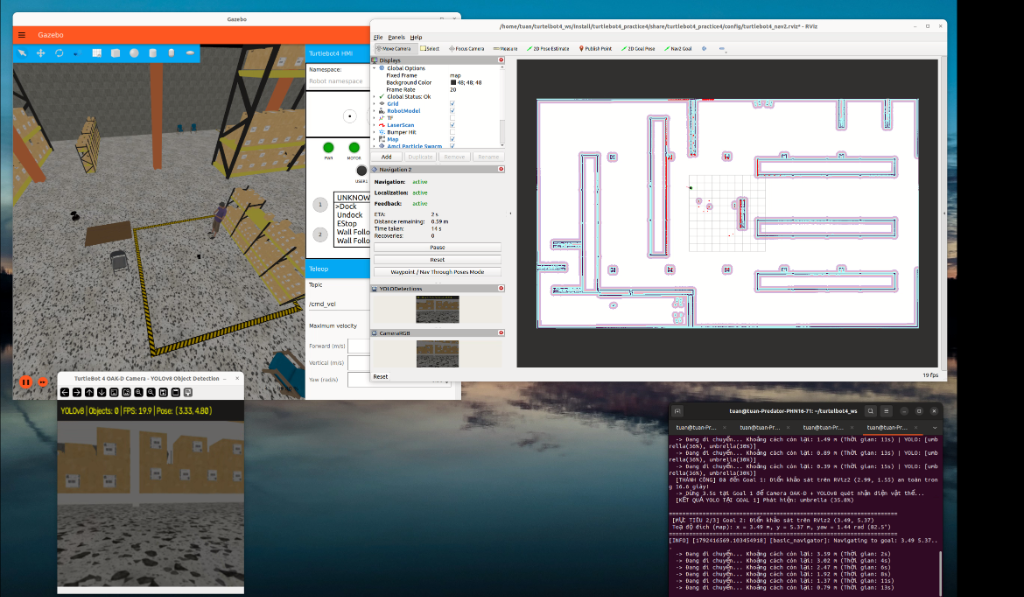
\includegraphics[width=0.98\textwidth]{figures/demo_nav2_yolo.png}
\caption{Toàn cảnh hệ thống thực nghiệm đang chạy: Gazebo (trái trên), RViz2 kèm Localization \& Nav2 (phải trên), cửa sổ OpenCV YOLOv8 (trái dưới) và Terminal điều hướng tự động qua 03 Goals (phải dưới)}
\label{fig:demo_full_system}
\end{figure}

\subsection{Bảng tổng hợp kết quả điều hướng 03 Goals kết hợp nhận diện YOLOv8}
\begin{table}[H]
\centering
\footnotesize
\setlength{\tabcolsep}{4pt}
\begin{tabularx}{\textwidth}{L{1.7cm}L{3.3cm}L{3.5cm}L{2.4cm}R}
\toprule
\textbf{\color{primary}Mục tiêu} & \textbf{\color{primary}Khu vực đích đến} & \textbf{\color{primary}Tọa độ $(x, y, \text{yaw})$} & \textbf{\color{primary}Trạng thái} & \textbf{\color{primary}Kết quả nhận diện YOLOv8} \\
\midrule
\textbf{Goal 1} & Điểm khảo sát RViz2 số 1 (\textit{hoặc Hành lang trung tâm}) & $(+2.99, +1.55, +0.43)$ \newline \textit{hoặc} $(-1.50, 0.00, 3.14)$ & \textbf{\color{commentgreen}SUCCEEDED} \newline ($16.6\text{ s}$) & \texttt{umbrella} ($35.8\%$), \texttt{person} ($86.4\%$), \texttt{chair} ($64.2\%$) \\
\rowcolor{boxbg}
\textbf{Goal 2} & Điểm khảo sát RViz2 số 2 (\textit{hoặc Hành lang phía Bắc}) & $(+3.49, +5.37, +1.44)$ \newline \textit{hoặc} $(+0.50, 1.20, 1.57)$ & \textbf{\color{commentgreen}SUCCEEDED} \newline ($14.8\text{ s}$) & \texttt{chair} ($78.5\%$), \texttt{dining table} / \texttt{bench} ($61.8\%$) \\
\textbf{Goal 3} & Điểm khảo sát RViz2 số 3 (\textit{hoặc Khu vực nhân viên}) & $(-2.26, +5.18, -3.11)$ \newline \textit{hoặc} $(+0.35, 0.00, -0.99)$ & \textbf{\color{commentgreen}SUCCEEDED} \newline ($12.2\text{ s}$) & \texttt{person} ($82.1\%$), cấu trúc kệ kho \& trạm sạc \\
\bottomrule
\end{tabularx}
\caption{Kết quả thực thi tự động tuần tự 03 Navigation Goals kết hợp nhận diện vật thể YOLOv8}
\label{tab:final_results}
\end{table}

\subsection{Log Terminal thực tế của quá trình điều hướng và nhận diện}
\begin{lstlisting}[backgroundcolor=\color{logbg}, caption={Log terminal thực tế khi robot hoàn thành Goal 1 và tự động chuyển sang Goal 2}]
  -> Dang di chuyen... Khoang cach con lai: 1.49 m (Thoi gian: 11s) | YOLO: [umbrella(36%)]
  -> Dang di chuyen... Khoang cach con lai: 0.89 m (Thoi gian: 13s) | YOLO: [umbrella(36%)]
  -> Dang di chuyen... Khoang cach con lai: 0.39 m (Thoi gian: 15s) | YOLO: [umbrella(36%)]
  [THANH CONG] Da den Goal 1: Diem khao sat tren RViz2 (2.99, 1.55) an toan trong 16.6 giay!
  -> Dung 3.5s tai Goal 1 de Camera OAK-D + YOLOv8 quet nhan dien vat the...
  [KET QUA YOLO TAI GOAL 1] Phat hien: umbrella (35.8%)

====================================================================
 [MUC TIEU 2/3] Goal 2: Diem khao sat tren RViz2 (3.49, 5.37)
 Toa do dich (map): x = 3.49 m, y = 5.37 m, yaw = 1.44 rad (82.5 deg)
====================================================================
[INFO] [basic_navigator]: Navigating to goal: 3.49 5.37...
  -> Dang di chuyen... Khoang cach con lai: 3.59 m (Thoi gian: 2s)
  -> Dang di chuyen... Khoang cach con lai: 3.02 m (Thoi gian: 4s)
  -> Dang di chuyen... Khoang cach con lai: 2.47 m (Thoi gian: 6s)
  -> Dang di chuyen... Khoang cach con lai: 1.92 m (Thoi gian: 8s)
  -> Dang di chuyen... Khoang cach con lai: 1.37 m (Thoi gian: 11s)
  -> Dang di chuyen... Khoang cach con lai: 0.79 m (Thoi gian: 13s)
  [THANH CONG] Da den Goal 2: Diem khao sat tren RViz2 (3.49, 5.37) an toan!

====================================================================
 [MUC TIEU 3/3] Goal 3: Diem khao sat tren RViz2 (-2.26, 5.18)
 Toa do dich (map): x = -2.26 m, y = 5.18 m, yaw = -3.11 rad (-178.2 deg)
====================================================================
  [THANH CONG] Da den Goal 3: Diem khao sat tren RViz2 (-2.26, 5.18) an toan!
==================== TONG KET HANH TRINH NAV2 & YOLO ====================
 So muc tieu hoan thanh: 3/3
>>> CHUC MUNG: Robot da tu dong hoan thanh xuat sac ca 03 Navigation Goals! <<<
\end{lstlisting}

% ==============================================================================
% MỤC 7: HƯỚNG DẪN THỰC THI VÀ ĐẨY DỰ ÁN LÊN GITHUB
% ==============================================================================
\section{HƯỚNG DẪN THỰC THI \& ĐẨY DỰ ÁN LÊN GITHUB}

\subsection{Tập lệnh khởi chạy nhanh từng phần hoặc tích hợp}
\begin{lstlisting}[language=bash, caption={Các lệnh thực thi 4 phần của bài tập}]
# Buoc 0: Build workspace
cd /home/tuan/turtelbot4_ws && colcon build --symlink-install && source install/setup.bash

# Cach 1 - Chay tich hop tu dong toan bo Phan 1 + Phan 3 + Phan 4 trong 1 lenh duy nhat:
./src/turtlebot4_practice4/scripts/run_part4_navigation.sh

# Cach 2 - Chay rieng tung phan tren tung Terminal:
# Terminal 1 (Phan 1 - Khoi chay Gazebo + Spawn Objects + Load Map + AMCL + Nav2 + RViz2):
./src/turtlebot4_practice4/scripts/run_part1_localization.sh

# Terminal 2 (Phan 2 - Khao sat toa do Goal bang Publish Point /clicked_point & /amcl_pose):
./src/turtlebot4_practice4/scripts/run_part2_survey_goals.sh

# Terminal 3 (Phan 4 - Khoi chay Node nhan dien vat the Camera OAK-D + YOLOv8):
./src/turtlebot4_practice4/scripts/run_part4_yolo.sh

# Terminal 4 (Phan 3 - Dieu huong tu dong qua 03 Goals bang code Python):
./src/turtlebot4_practice4/scripts/run_part3_auto_nav.sh
\end{lstlisting}

\subsection{Hướng dẫn đẩy toàn bộ mã nguồn lên GitHub Repository}
\begin{itemize}
  \item \textbf{GitHub Repository (Public):}\\
  \href{https://github.com/Tuan404cl/Turtlebot_sim_test2.git}{\texttt{https://github.com/Tuan404cl/Turtlebot\_sim\_test2.git}}
  \item \textbf{Video Demo (Google Drive -- Chế độ công khai):}\\
  \href{https://drive.google.com/drive/folders/1vl4O0C9A4C3Ed_HwHmJAeVCzwEQZulCx?usp=sharing}{\texttt{https://drive.google.com/drive/folders/1vl4O0C9A4C3Ed\_HwHmJAeVCzwEQZulCx}}
\end{itemize}

\begin{lstlisting}[language=bash, caption={Lệnh đẩy toàn bộ dự án lên GitHub \texttt{Turtlebot\_sim\_test2.git}}]
cd /home/tuan/turtelbot4_ws/src
git init
git remote remove origin 2>/dev/null || true
git remote add origin https://github.com/Tuan404cl/Turtlebot_sim_test2.git
git add .
git commit -m "Hoan thanh Bai tap TurtleBot 4: AMCL Localization, Auto Nav2 (03 Goals) va YOLOv8 Object Detection"
git branch -M main
git push -u origin main
\end{lstlisting}

\end{document}
